\documentclass{beamer}
\usepackage{listings}
\lstset{
%language=C,
frame=single, 
breaklines=true,
columns=fullflexible
}
\graphicspath{./figures/}
\usepackage{subcaption}
\usepackage{url}
\usepackage{tikz}
\usepackage{tkz-euclide} % loads  TikZ and tkz-base
%\usetkzobj{all}
\usetikzlibrary{calc,math}
\usepackage{float}
\newcommand\norm[1]{\left\lVert#1\right\rVert}
\renewcommand{\vec}[1]{\mathbf{#1}}
\usepackage[export]{adjustbox}
\usepackage[utf8]{inputenc}
\usepackage{amsmath}
\providecommand{\pr}[1]{\ensuremath{\Pr\left(#1\right)}}
\providecommand{\brak}[1]{\ensuremath{\left(#1\right)}}
\providecommand{\cbrak}[1]{\ensuremath{\left\{#1\right\}}}
\usetheme{Boadilla}

\title{Central limit theorem and Application}
\author{Ganesh Bombatkar-CS20BTECH11016}

\institute{}
\date{\today}
\begin{document}


\begin{frame}
\titlepage
\end{frame}

\section{Prerequisites}
\begin{frame}{PREREQUISITES}
    \begin{enumerate}
        \item Normal distribution
        \item Central limit theorem
        \item Poisson distribution and some  properties
    \end{enumerate}
\end{frame}
\subsection{Normal distribution}
\begin{frame}{\textbf{Normal distribution}}
    Normal (Gaussian) distribution it's probability density given by
    \begin{align}
        F(x)=& \frac{1}{\sqrt{2\pi \sigma^2}} e^{-\frac{{\brak{x-\mu}}^2}{2\sigma^2}}
    \end{align}
    The parameter $\mu$ and $\sigma$ are mean and standard deviation respectively
    \begin{columns}[onlytextwidth]
    \column{0.5\textwidth}
    \begin{block}{Standard normal distribution}
       Normal distribution with $\mu=0$ and $\sigma^2=1$ is Standard normal distribution . It's PDF denoted by $\varphi$
       \begin{align}
           \varphi = \frac{1}{\sqrt{2\pi}} e^{-\frac{x^2}{2}}
       \end{align}
    \end{block}
    \column{0.5\textwidth}
    \begin{figure}
        \centering
        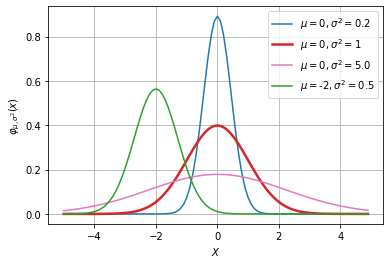
\includegraphics[scale=0.4]{figures/norm.png}
        %\caption{Caption}
        \label{fig:my_label}
    \end{figure}
    \end{columns}
\end{frame}

\subsection{central limit theorem}
\begin{frame}{\textbf{Central limit theorem}}
    { \small
    When independent random variables are added, their properly normalized sum tends toward a normal distribution even if the original variables themselves are not normally distributed}%
    \begin{block}{}
       {\small Let  $X_1 ,X_2 ,..,X_n$ are i.i.d and $\hat X=\frac{1}{n}\sum \limits_{i=1}^{n}X_i $ has mean $\mu $ and variance $\sigma^2$
       \begin{align}
        Z=\lim \limits_{n \to \infty } \frac{\hat X - \mu }{\sigma }    
       \end{align}
        then $Z$ approaches standard normal distribution with $\mu = 0$ and $\sigma^2 = 1$  }%
    \end{block}
    \begin{columns}[onlytextwidth]
    \column{0.33\textwidth}
    \begin{figure}
        \centering
        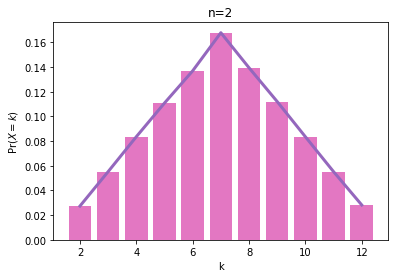
\includegraphics[scale=0.22]{figures/CLT/n=2.png}
        %\caption{Caption}
        \label{fig:my_label}
    \end{figure}
    \column{0.33\textwidth}
    \begin{figure}
        \centering
        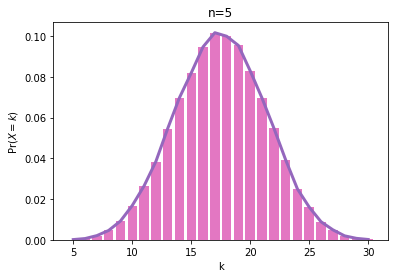
\includegraphics[scale=0.22]{figures/CLT/n=5.png}
        %\caption{Caption}
        \label{fig:my_label}
    \end{figure}
    % \column{0.22\textwidth}
    % \begin{figure}
    %     \centering
    %     \includegraphics[scale=0.22]{figures/CLT/n=10.png}
    %     %\caption{Caption}
    %     \label{fig:my_label}
    % \end{figure}
    \column{0.33\textwidth}
    \begin{figure}
        \centering
        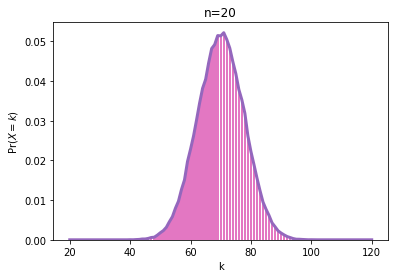
\includegraphics[scale=0.22]{figures/CLT/n=20.png}
        %\caption{Caption}
        \label{fig:my_label}
    \end{figure}
    \end{columns}
    \begin{center}
          {\tiny plots to show   Central limit theorem on event of rolling $n$ dices}%
    \end{center}
\end{frame}

\subsection{Poisson distribution}
\begin{frame}{\textbf{Poisson distribution}}
    % 
    Poisson distribution is used to model the number of events occurring within a given time interval
    \begin{block}{}
    \begin{align}
        \pr{X=k}\,\,=&\,\,\frac{e^{-\lambda} \lambda^k}{k!}  \quad \text{ for } k = 0,1,2,...
    \end{align}
    \end{block}
    Here $\lambda$ is shape parameter indicating average number of events in given time interval
    \begin{figure}
        \centering
        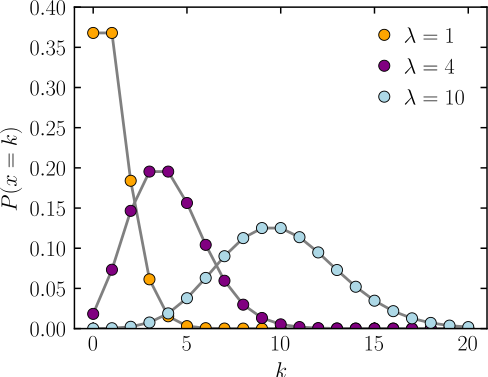
\includegraphics[width=0.5\textwidth,height=0.3\textwidth]{figures/poisson.png}
        %\caption{Caption}
        \label{fig:my_label}
    \end{figure}
\end{frame}

\subsubsection{Properties}
\begin{frame}{Summation of Poisson random variable}
    \begin{block}{}
       Let $X$ and $Y$ are independent Poisson random variables with parameter $\alpha$ and $\beta$ respectively then $Z=X+Y$ is a Poisson random variable with parameter $\alpha+\beta$
    \end{block}
    \begin{block}{proof:}
    {\small
        \begin{align}
            \pr{Z=z}=&\sum_{k=0}^{z} \pr{X=k}\times \pr{Y=z-k}
            \\=&\sum_{k=0}^{z}\frac{e^{-\alpha} \alpha^k}{k!}\times \frac{e^{-\beta} \beta^{z-k}}{\brak{z-k}!} 
            % \\=&\frac{e^{-\brak{\alpha+\beta}} }{k!}  \sum_{k=0}^{z}{\binom{z}{k} \alpha^k\beta^\brak{z-k}}
            \\=& \frac{e^{-\brak{\alpha +\beta}}}{z!} \sum_{k=0}^{z}\binom{z}{k}\alpha^k \beta^{z-k}
            \\=&\frac{e^{-\alpha + \beta} \brak{\alpha + \beta}^z}{z!} 
        \end{align}
    }%
    \end{block}
\label{addative_property}
\end{frame}
\section{Question}
\begin{frame}{\textbf{Question:}}
    \begin{block}{\textbf{UGC/MATH (math Dec 2017), Q.107}}
    For $n \geq 1$, let $X_n$ be a Poisson random  variable with mean $n^2$.
 Which of the following's are equal to
 $\displaystyle{\frac{1}{\sqrt{2\pi}} \int \limits_2^{\infty} e^{-x^2/2}\,dx}$
 \begin{enumerate}
    \item $\lim \limits_{n \to \infty} $ \pr{X_n > (n+1)^2}
    \item $\lim \limits_{n \to \infty} $ \pr{X_n \leqslant (n+1)^2}
    \item $\lim \limits_{n \to \infty} $ \pr{X_n<(n-1)^2}
    \item $\lim \limits_{n \to \infty} $ \pr{X_n<(n-2)^2}
\end{enumerate}
    \end{block}
\end{frame}

\section{Solution}
\begin{frame}{\textbf{Solution:}}
    $X_n$ is a Poisson random variable with parameter $n^2$ and 
    Let $Y_i$ be a Poisson random variable with parameter $1$, for $i$ $\in$ $\brak{1,n^2}$
\begin{block}{
By additive property of Poisson distribution}
\begin{align}
   { \sum \limits_{i=1}^{n^2} Y_i = X_n   }  
\end{align}
\end{block}
\begin{block}{
By central limit theorem }

\begin{align}
    \lim  \limits_{n \to \infty} \frac{Y_1+Y_2+..+Y_{n^2} - n^2}{n} = \mathcal{N}(0,1)
    \\ \implies \lim  \limits_{n\to \infty} \frac{X_n-n^2}{n} = \mathcal{N}\brak{0,1}
\end{align}
Here, $\mathcal{N}\brak{0,1}$ is normal distribution with zero mean and unit variance
\end{block}
\end{frame}

\begin{frame}{}
\begin{block}{}
    \begin{align}
    \pr{X_n>k} =& \pr{\frac{X_n-n^2}{n}>\frac{k-n^2}{n}}
    \\=& \pr{\mathcal{N}\brak{0,1}>\frac{k-n^2}{n}}
    \\ =& Q\brak{\frac{k-n^2}{n}}
    \label{eq-cdf}
    \end{align}
\end{block}
\end{frame}

\begin{frame}{}
    \begin{block}{}
{\small
    \begin{align}
    Q\brak{X}=1-Q\brak{-x}
    \end{align}
    \begin{align*}
    \because \,{\frac{1}{\sqrt{2\pi}} \int \limits_{-x}^{\infty} e^{-x^2/2}\,dx}\,=\,{\frac{1}{\sqrt{2\pi}} \int \limits_{-\infty}^x e^{-x^2/2}\,dx}
    \quad \text{and} \quad \frac{1}{\sqrt{2\pi}} \int \limits_{-\infty}^{\infty} e^{-x^2/2}\,dx =1
    \end{align*}
}%
\end{block}

\begin{block}{}
    \begin{align}
    \frac{1}{\sqrt{2\pi}} \int \limits_2^{\infty} e^{-x^2/2}\,dx=& Q\brak{2}
    \\\frac{1}{\sqrt{2\pi}} \int \limits_2^{\infty} e^{-x^2/2}\,dx=&1-Q\brak{-2}
    \end{align}
\end{block}
\end{frame}

\begin{enumerate}
\subsection{Option 1}
\begin{frame}{}
\begin{block}{\item  $\lim \limits_{n \to \infty} $ \pr{X_n > (n+1)^2}}
\begin{align}
    \lim \limits_{n \to \infty} \pr{X_n > (n+1)^2} =& \lim \limits_{n \to \infty}Q \brak{\frac{(n+1)^2-n^2}{n}}
    \\=&Q\brak{2}
\end{align}
$\mathbf{\therefore}$ \textbf{Option 1 is correct}
\end{block}
\end{frame}

\begin{frame}{}
\subsection{Option 2}
\begin{block}{
\item $\lim \limits_{n \to \infty} $ \pr{X_n \leqslant (n+1)^2}}
\begin{align}
    \lim \limits_{n \to \infty}  \pr{X_n \leqslant (n+1)^2} =&1-\lim \limits_{n \to \infty}  \pr{X_n > (n+1)^2}
    \\=&1- \lim \limits_{n \to \infty}Q \brak{\frac{(n+1)^2-n^2}{n}}
    \\=&1- Q \brak{2}
    \\ =& Q\brak{-2} > Q\brak{2}
\end{align}
$\mathbf{\therefore}$ \textbf{Option 2 is incorrect}
\end{block}
\end{frame}

\begin{frame}{}
\subsection{Option 3}
\begin{block}{
\item $\lim \limits_{n \to \infty} $ \pr{X_n < (n-1)^2}}
\begin{align}
    \lim \limits_{n \to \infty}  \pr{X_n < (n-1)^2} =& 1-\lim \limits_{n \to \infty}  \pr{X_n \geq (n-1)^2}
    \\=&1-\lim \limits_{n \to \infty}Q \brak{\frac{(n-1)^2-n^2}{n}}
    \\=& 1-Q \brak{-2}
    \\=& Q\brak{2}
\end{align}
$\mathbf{\therefore}$ \textbf{Option 3 is also correct}
\end{block}
\end{frame}

\begin{frame}{}
\subsection{Option 4}
\begin{block}{
\item $\lim \limits_{n \to \infty} $ \pr{X_n < (n-2)^2}}
\begin{align}
    \lim \limits_{n \to \infty}  \pr{X_n < (n-2)^2} =& 1-\lim \limits_{n \to \infty}  \pr{X_n \geq (n-2)^2}
    \\=&1-\lim \limits_{n \to \infty}Q \brak{\frac{(n-2)^2-n^2}{n}}
    \\=&1- Q \brak{-4}
    \\=& Q\brak{4} < Q \brak{2}
\end{align}
\newpage
$\mathbf{\therefore}$ \textbf{Option 4 is incorrect}
\end{block}
\end{frame}
\end{enumerate}

\end{document}